\section{System Overview}
Through the system overview diagram, in figure \ref{fig:system_overview}, it is possible to identify the main modules of the system to be developed, and how they interact. We can divide the system into two subsystems: the local system, which represents a lamp post, and the remote system, that allows interaction with the system users.

\begin{figure}[ht]
	\centering
	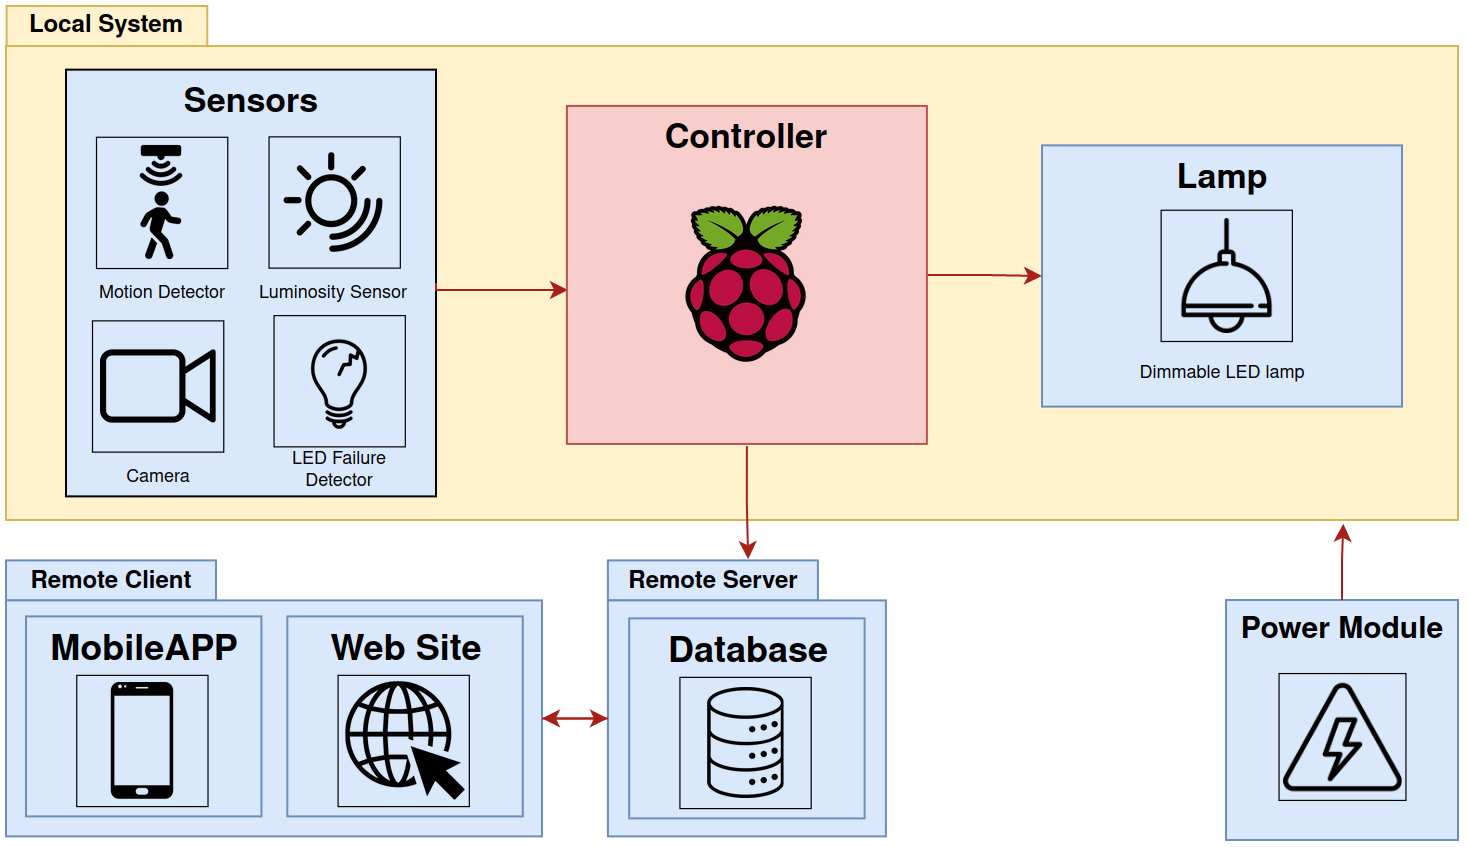
\includegraphics[width=1\textwidth]{system_overview}
	\caption{System Overview Diagram.}
	\label{fig:system_overview}
\end{figure}

The local system is composed of sensors, a controller and a lamp. Regarding the sensors, there will be a motion detector, to allow the detection of movement in the vicinity of the pole, a luminosity sensor, to detect the light conditions of the pole’s surroundings, a camera to find empty parking spots and a LED failure detector to know if the LED lamp is working. The controller, the Raspberry Pi, through sensors information, controls the luminosity of the lamp and communicates through the internet with a remote server, using the Wi-Fi module. Each lamp post communicates with the neighbor posts to turn on the lights dinamically, so the local system communicates with other local systems, also through the Wi-Fi module.

The remote system is composed by the remote server and the remote client. The remote server consists of a database that stores all information about each lamp post location and operating status. This information can be accessed through a mobile application by the operator  responsible for the street lights network, in order to carry out the necessary maintenance of the lamp of each pole. Furthermore, the operator when installing a new lamp post can add its location to the database, using the mobile application. In addition, the database stores information on available parking spaces. When a user, a car driver, wants to know where there are empty parking places, he can access a website that informs him of the location of the empty parking spaces.

Knowing that the public lighting network is directly related to the electrical network, this will be used to power each local system.

\section{System Requirements and Constraints}
In order for the system to have the desired performance, these requirements and constraints must be respected:

\subparagraph{Functional Requirements}
\begin{itemize}
	\item Sensors data acquisition				
	\item Motion detection
	\item Control of a street lamp
	\item Wi-Fi communication
	\item Empty parking spots detection
	\item Manage system information through a mobile application
	\item Add lamp post location through a mobile application
	\item Access available parking spots location through a web site
\end{itemize}

\subparagraph{Non-Functional Requirements}
\begin{itemize}
	\item User friendly mobile application and web site
	\item Ambient luminosity sensing
	\item Lower power consumption than actual street lights
	\item Soft Real-Time Embedded System
\end{itemize}

\subparagraph{Technical Constraints}
\begin{itemize}
	\item Buildroot
	\item C and C++ 
	\item Device Drivers
	\item Linux
	\item Raspberry Pi
	\item \ac{cps}
	\item Makefiles
	\item Pthreads
\end{itemize}

\subparagraph{Non-Technical Constraints}
\begin{itemize}
	\item Two members team
	\item Project deadline at the end of the semester
	\item Low budget
\end{itemize}

\section{System Architecture}
Using the system overview diagram information, one can describe the system in two different architectures. Hardware architecture, as how the hardware modules interfaces with itself, and what are the physical components of the system, and software architecture, which details how the information is processed among different software layers.

\clearpage

\subsection{Hardware Architecture}
In figure \ref{fig:hw_arch}, one can see the diagram that represents the physical connections of the system. The Raspberry Pi is the main component in the system, processing all the information given by the sensors, via \ac{gpio} pins and \ac{csi} for the camera. The communication with the Wi-Fi module is straightforward since its built-in into the Raspberry-Pi.
%, and also controlling the \ac{led} lamp brightness. 

The power of all system components comes from the power grid and, through an AC/DC converter, will power the Raspberry Pi and its associated sensors.

In order to power the lamp and at the same time control its brightness, a driver is used, taking the controller output, a \ac{pwm} signal, and system power as inputs. 

\begin{figure}[ht]
	\centering
	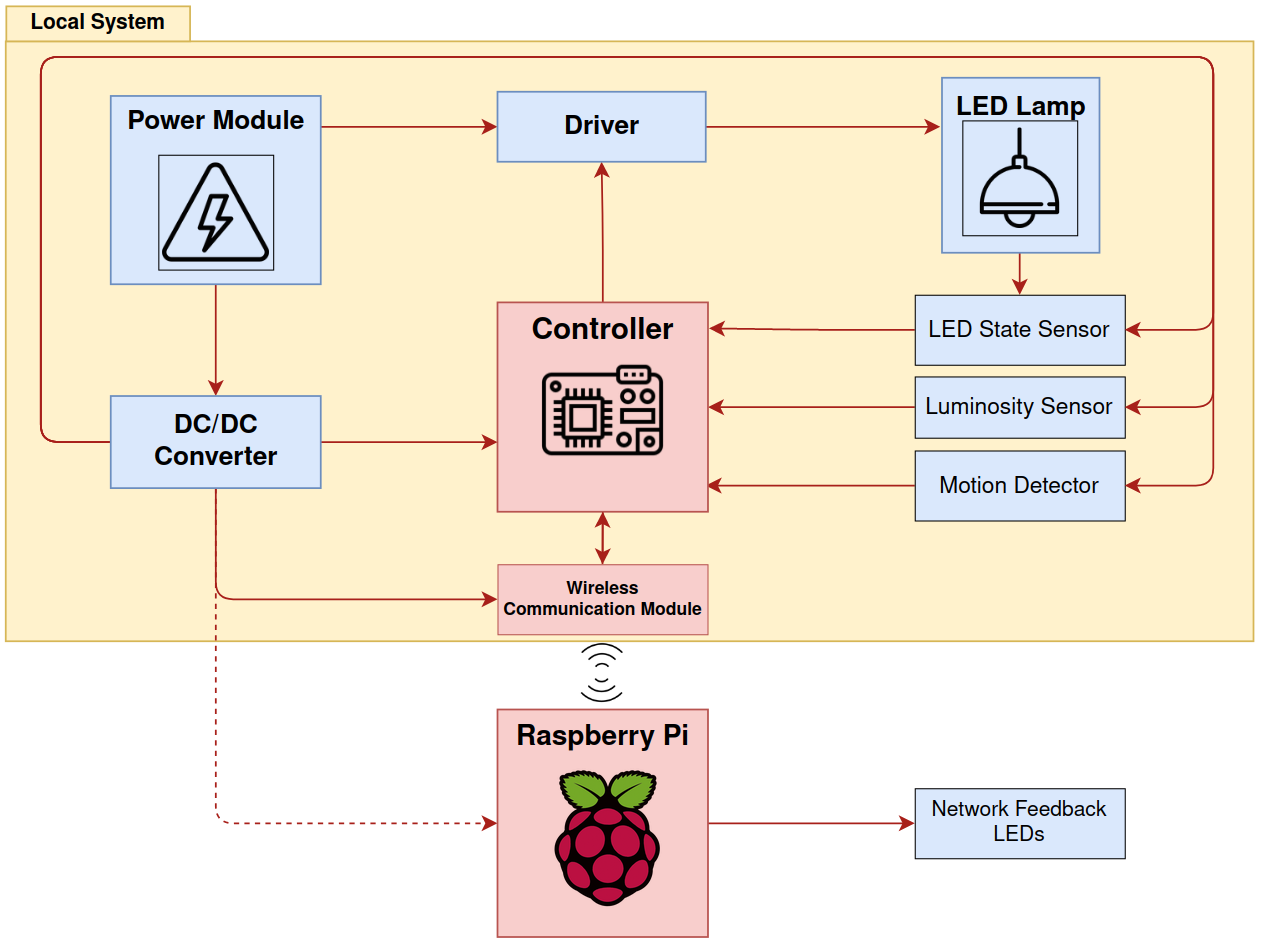
\includegraphics[width=1\textwidth]{hw_arch}
	\caption{Hardware Architecture Diagram.}
	\label{fig:hw_arch}
\end{figure}

\subsection{Software Architecture}
The software architecture is divided into three layers:

\begin{itemize}
	\item The \textbf{Operating System} layer, which is composed by the Operating System drivers and Board Support Packages;
	\item The \textbf{Middleware} layer, which includes software for abstracting the lower level layer packages. It works as a pipe since it links two applications, in different layers, so that data can be easily transmitted;
	\item The \textbf{Application} layer, where the core functionality of the program is built, with a resource for the API's in the lower level layers.
\end{itemize}

As shown in figure \ref{fig:sw_arch}, the operating system layer is composed by the sensor drivers, such as the LED Failure Sensor, the Luminosity Sensor, the Motion Detector which uses \ac{gpio} drivers, the camera, that uses \ac{csi} drivers and also the Wi-Fi Communication driver. In the middleware layer are the tools needed to process the images from the camera, to multitasking, using PThreads execution model, to acquire data from sensors and to communicate via Wi-Fi with the remote server. Finally, the application layer manages the system database, as well as the \ac{gui}, that is the mobile application and the web site, and also all communications with the neighbor street poles.

\begin{figure}[ht]
	\centering
	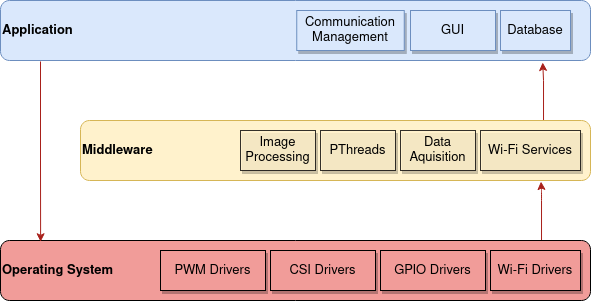
\includegraphics[width=1\textwidth]{sw_arch}
	\caption{Software Architecture Diagram.}
	\label{fig:sw_arch}
\end{figure}